\section{Overview}

The most important parts of this lecture are the following:

\begin{enumerate}
\item \textbf{Richardson's Extrapolation}: A method for obtaining higher order
  accuracy from lower order formulas. link: \ref{sec:richardson_extrapolation}
  \begin{enumerate}
    \item \ref{sec:building_the_extrapolation_table} illustrates the procedure of
      building the richardson extrapolation table.
    \item \ref{sec:richardson_extrapolation_example} illustrates the use of
      Richardson's Extrapolation to obtain a higher order approximation to the
      integral of $\sin x$.
  \end{enumerate}
\item \textbf{Numerical Integration}: A method for evaluating the definite
  integral of a function that has no explicit antiderivative or whose antiderivative
  is not easy to obtain. link: \ref{sec:numerical_integration}
  \begin{enumerate}
    \item \ref{sec:two_point_integration} illustrates the procedure of using a
      2 point integration formula.
    \item \ref{sec:weighted_mean_value_theorem} illustrates the procedure of
      using the weighted mean value theorem for integrals.
    \item \ref{sec:three_point_integration} illustrates the procedure of using a
      3 point integration formula.
  \end{enumerate}
\end{enumerate}

\pagebreak
\section{Richardson's Extrapolation (C4*1-17.10)}\label{sec:richardson_extrapolation}

When the error depends on some parameter such as the step size $h$ and the
dependency is predictable, we can often derive higher order accuracy from low
order formulas. To illustrate the procedure, assume we have an approximation
$N(h)$ to some quantity $M$. Assume this approximation has an order $h$
truncation error and that we know the expression for the first few terms of the
trunction error,

\begin{equation}
M = N(h) + k_1h + k_2h^2 + k_3h^3 + \dots
\label{eq:*}
\end{equation}

\noindent where the $k_i$'s are constants, $h$ is a positive parameter and
$N(h)$ is an $O(h)$ approximation to $M$. We can repeat the calculation with a
parameter $\frac{h}{2}$:

\begin{equation}
M=N\left(\frac{h}{2}\right) + \frac{k_1}{2}h + \frac{k_2}{4}h^2 + \frac{k_3}{8}h^3 + \dots
\label{eq:**}
.\end{equation}

We want to obtain a higher order method by using some combination of these
results. 
Subtracting \eqref{eq:*} from twice \eqref{eq:**} gives:

\begin{equation}
  M = \left[2N\left(\frac{h}{2}\right) - N(h)\right] + k_2\left(\frac{h^2}{2} 
  - h^2\right) + k_3 \left(\frac{h^3}{4}-h^3\right) + \dots
  \label{eq:?}
\end{equation}

\noindent
which is an $O(h^2)$ approximation formula for $M$. For ease of notiation, 

\[
\text{Let } N_2(h) = 2N\left(\frac{h}{2}\right) - N(h)
.\]

% \begin{minipage}{\textwidth}
\noindent
Generally, if $M$ can be written as

\[
  M = N(h) + \sum_{j=1}^{m-1} K_j h^j + O(h^m),
.\]

\noindent
then for each $j = 2, 3, \dots, m$, we have an $O(h^j)$ approximation of the form

\[
  N_j(h) = N_{j-1} \left(\frac{h}{2}\right) + \frac{N_{j-1} \left(\frac{h}{2}\right) - N_{j-1}(h)}{2^{j-1} - 1}.
.\]
% \end{minipage}

In practice, because of how $N_j$ is defined, higher order approximations can 
be systematically derived from lower order approximations.

\subsubsection{Building the Extrapolation Table (18.1)}\label{sec:building_the_extrapolation_table}

\begin{center}
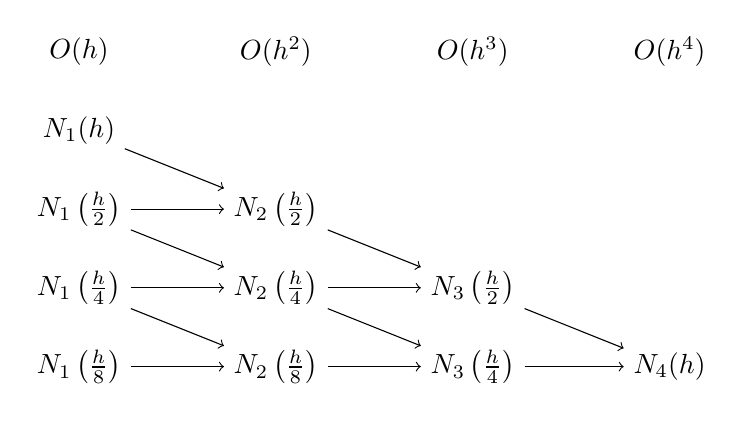
\begin{tikzpicture}[node distance=1cm, font=\sffamily]
  % Nodes
  \node (Oh) {$O(h)$};
  \node[right of=Oh, xshift=1.5cm] (Oh2) {$O(h^2)$};
  \node[right of=Oh2, xshift=1.5cm] (Oh3) {$O(h^3)$};
  \node[right of=Oh3, xshift=1.5cm] (Oh4) {$O(h^4)$};

  % First column nodes
  \node[below of=Oh] (N1h) {$N_{1}(h)$};
  \node[below of=N1h] (N1h2) {$N_{1}\left(\frac{h}{2}\right)$};
  \node[below of=N1h2] (N1h4) {$N_{1}\left(\frac{h}{4}\right)$};
  \node[below of=N1h4] (N1h8) {$N_{1}\left(\frac{h}{8}\right)$};

  % Second column nodes
  \node[right of=N1h2, xshift=1.5cm] (N2h2) {$N_{2}\left(\frac{h}{2}\right)$};
  \node[right of=N1h4, xshift=1.5cm] (N2h4) {$N_{2}\left(\frac{h}{4}\right)$};
  \node[right of=N1h8, xshift=1.5cm] (N2h8) {$N_{2}\left(\frac{h}{8}\right)$};

  % Third column nodes
  \node[right of=N2h4, xshift=1.5cm] (N3h2) {$N_{3}\left(\frac{h}{2}\right)$};
  \node[right of=N2h8, xshift=1.5cm] (N3h4) {$N_{3}\left(\frac{h}{4}\right)$};

  % Fourth column node
  \node[right of=N3h4, xshift=1.5cm] (N4h) {$N_{4}(h)$};

  % Arrows
  \draw[->] (N1h2) -- (N2h2);
  \draw[->] (N1h2) -- (N2h4);
  \draw[->] (N1h) -- (N2h2);
  \draw[->] (N1h4) -- (N2h4);
  \draw[->] (N1h8) -- (N2h8);
  \draw[->] (N2h2) -- (N3h2);
  \draw[->] (N3h2) -- (N4h);
  \draw[->] (N1h4) -- (N2h8);
  \draw[->] (N2h4) -- (N3h4);

  \draw[->] (N2h4) -- (N3h2);
  \draw[->] (N2h8) -- (N3h4);
  

  \draw[->] (N3h4) -- (N4h);
\end{tikzpicture}
\end{center}

The cost of building the extrapolation table is $O(n)$ where $n$ is the inverse 
degree of the error term $(O(h^n))$. Each subsequent iteration of $N$ is defined
solely by its previous iteration, therefore, the cost of building the
extrapolation is the number of initial calculations of $N_1$ required to build
out the table. Some pitfalls of this approach is that the calculation of
$N_{j+1}$ requires a subtraction of two numbers that get closer and closer as
the degree of the error term increases. This is a problem for higher order
calculations, as you may run out of precision and introduce substantial machine
error.

Extrapolation can be used whenever the truncation error for a formula has the
form

\[
  \sum_{j=1}^{m-1} K_j h^{\alpha_j} + O(h^{\alpha_m})
.\]

\noindent
for constants $K_J$ and $\alpha_1 < \alpha_2 < \dots < \alpha_m$.

\subsubsection{When $N_j(h)$ is an $O(h^{2j})$ approximation}\label{sec:richardson_extrapolation_when_n_j_is_o_h_2j}
Suppose $N_j(h)$ is an $O(h^{2j})$ approximation of $M$. Then, from the
definition:

\begin{align}
  M &= N_j(h) + O(h^{2j}) \qquad \text{we add another term of } M \text{:} \\
    &= N_j(h) + k_j(h^{2j}) + O(h^{2j+2}) \label{eq:diamond} \\
    &= N_j(\frac{h}{2}) + k_jh^{2j} + O(h^{2j+2}) \label{eq:2diamond}
\end{align}

$2^{2j}$ \eqref{eq:diamond} $-$ \eqref{eq:2diamond} gives:

\begin{equation*}
  M = N_j(\frac{h}{2}) + \frac{N_j(\frac{h}{2})-N_j(h)}{2^{2j-1}} + O(h^{2j+2})
\end{equation*}

\[
  \boxed{\therefore 
    N_{j+1}(h) \equiv N_j\left(\frac{h}{2}\right) 
    + \frac{N_j\left(\frac{h}{2}\right)-N_j(h)}{4^{j-1}}
  }
.\]

\noindent
is an $O(h^{2j+2})$ approximation of $M$. Then, the table becomes

\begin{center}
  \centering
  \begin{tabular}{cccc}
    $O(h^2)$ & $O(h^4)$ & $O(h^6)$ & $O(h^8)$
  \end{tabular}
\end{center}

\subsection{Richardson's Extrapolation Example (18.1)}\label{sec:richardson_extrapolation_example}

\Ex The following data gives approximations to the integral 

\begin{equation}
  M = \int_0^\infty \sin x \, dx
\end{equation}

\begin{align*}
N_{1}\left(\frac{h}{2}\right) = 1.570796,\quad 
N_{1}\left(\frac{h}{2}\right) = 1.896119\\[6pt]
N_{1}\left(\frac{h}{4}\right) = 1.974232,\quad 
N_{1}\left(\frac{h}{8}\right) = 1.993570
\end{align*}

Assuming 

\[
M = N_1(h) + K_1h^2 + K_2h^4 + k_3h^6 + k_4h^8 + O(h^{10})
.\]

construct an extrapolation table to determine $N_4(h)$.

\soln (from text)

\pagebreak
\section{Numerical Integration (18.4)}\label{sec:numerical_integration}

We often need to evaluate the definite integral of a function that has no
explicit antiderivative or whose antiderivative is not easy to obtain. The usual
strategy in developing formulas for numerical integration is similar to that for
numerical differentiation. We pass a polynomial through points defined by the
function and then integrate this polynomial approximation for the function. This
permist us to use a function known only as a table of values. We get an
expression for the error by integrating the error for our interpolating
polynomial. As we progress, we will eventually turn to splitting our function
into sub-intervals and using methods similar to spline interpolation to
integrate each sub-interval.

\subsection{2-Point Integration Formula (18.5)}\label{sec:two_point_integration}

Suppose we use a 2 point integration formula:

\begin{center}
  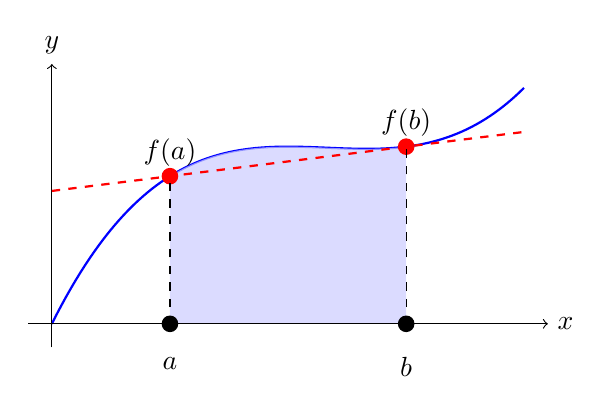
\begin{tikzpicture}[scale=3]
    % Define the function
    \def\f(#1){0.5*(#1)^3 - 1.75*(#1)^2 + 2*(#1)}

    % Define points
    \def\a{0.5}
    \def\b{1.5}

    % Draw the function
    \draw[thick, blue, domain=0:2, samples=100] plot (\x, {\f(\x)});
    % \draw[thick, red, domain=0:2, samples=100] plot (\x, )


    % Shade region between a and b
    \fill[blue!20, opacity=0.7] (\a,0) -- plot[domain=\a:\b, samples=50] (\x, {\f(\x)}) -- (\b,0) -- cycle;

    % Draw axes
    \draw[->] (-0.1,0) -- (2.1,0) node[right] {\(x\)};
    \draw[->] (0,-0.1) -- (0,1.1) node[above] {\(y\)};

    % Dots at the required points
    \foreach \x in {\a, \b} {
        \fill (\x, 0) circle (1pt);
    }
    \foreach \x in {\a, \b} {
      \fill[red] (\x, {\f(\x)}) circle (1pt);
    }

    \draw[dashed] (\a,0) -- (\a, {\f(\a)});
    \draw[dashed] (\b,0) -- (\b, {\f(\b)});
    % \draw[dashed] (\c,0) -- (\c, {\f(\c)});
    \draw[thick, red, dashed, domain=0:2, samples=100] plot (\x, {0.75 + 0.125 * (\x - 1.5)}); % Tangent line

    % Labels for the points
    \node[below] at (\a, -0.1) {\(a\)};
    \node[below] at (\b, -0.1) {\(b\)};
    % \node[below] at (\c, 0) {$\displaystyle\frac{a+b}{2}$};
    \node[above] at (\a, {\f(\a)}) {\(f(a)\)};
    \node[above] at (\b, {\f(\b)}) {\(f(b)\)};
  \end{tikzpicture}
\end{center}


Let $x_0 = a$, $x_1 = b$, $h=b-1$

The linear Lagrange polynomial passing through $(x_0, f(x_0))$ and $(x_1, f(x_1))$ 
is 

\[
P_1(x) = \frac{(x-x_1)(x-x_0)}{f(x_0)} + \frac{(x-x_0)}{(x_1-x_0)} f(x_1)
.\]

and

\begin{align*}
  \int_a^b f(x) \, dx &= \int_{x_0}^{x_1} P_1(x) \, dx +\frac{1}{2}\int_{x_0}^{x}
  f''\left(\xi(x)\right)(x - x_0)(x - x_1)\,dx \\
  &=  \left.\frac{(x - x_1)^2}{2(x_0 - x_1)}f(x_0) + \frac{(x - x_0)^2}{2(x_1 - x_0)}f(x_1)\right|_{x_0}^{x_1} + \text{error}\\[10pt]
  &= \frac{h}{2}\left(f(x_0) + f(x_1)\right) + \text{error}.
\end{align*}

To evaluate the error we will need the \textbf{Weighted Mean Value Theorem for
Integrals}.

\subsubsection{Weighted Mean Value Theorem for Integrals (18.6)}\label{sec:weighted_mean_value_theorem}

If $f\in C[a,b]$, the Riemann Integral of $g$ exists on $[a,b]$ and $g(x)$ does
not change sign on $[a,b]$ then there exists a number $c \in (a,b)$ such that

\[
  \int_a^b f(x) g(x) \, dx = f(c) \int_a^b g(x) 
.\]

\hrule

\begin{align*}
  \text{error} &= \frac{1}{2}\int_{x_0}^{x_1} f''\left(\xi(x)\right)(x - x_0)(x - x_1)\,dx \\
               &= \frac{1}{2} f''(\xi)\int_{x_0}^{x_1}(x - x_0)(x - x_1)\,dx \quad\text{[$\xi$ some number in $(x_0,x_1)$]}\\[6pt]
               &= \frac{1}{2}f''(\xi)\left[\frac{x^3}{3}-\frac{(x_1 + x_0)}{2}x^2+x_0x_1 x\right]_{x_0}^{x_1}\\[6pt]
               &= -\frac{h^3}{12}f''(\xi)
\end{align*}


\[
  \text{Thus } \boxed{
    \int_a^b f(x) \, dx = \frac{h}{2} \left[f(x_0) + f(x_1)\right] -
    \frac{h^3}{12} f''(\xi)
  }
\]

This is known as the \textbf{Trapezoid Rule} since the integral is approximated
by the area of a trapezoid.

\subsection{Three Point Integration Formula (18.7)}\label{sec:three_point_integration}
We might also consider a 3 point integration formula based on equally spaced
points:

\begin{center}
  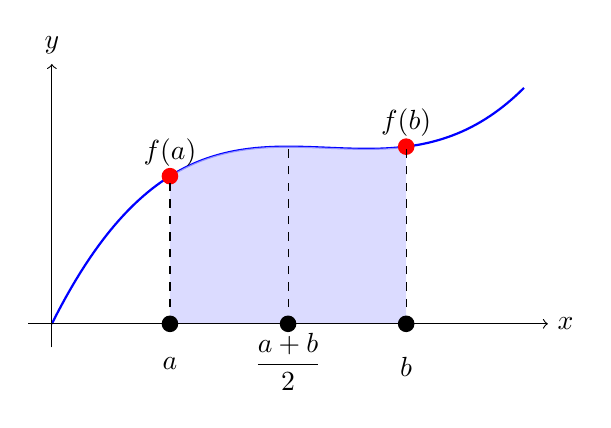
\begin{tikzpicture}[scale=3]
    % Define the function
    \def\f(#1){0.5*(#1)^3 - 1.75*(#1)^2 + 2*(#1)}

    % Define points
    \def\a{0.5}
    \def\b{1.5}
    \def\c{1}

    % Draw the function
    \draw[thick, blue, domain=0:2, samples=100] plot (\x, {\f(\x)});

    % Shade region between a and b
    \fill[blue!20, opacity=0.7] (\a,0) -- plot[domain=\a:\b, samples=50] (\x, {\f(\x)}) -- (\b,0) -- cycle;

    % Draw axes
    \draw[->] (-0.1,0) -- (2.1,0) node[right] {\(x\)};
    \draw[->] (0,-0.1) -- (0,1.1) node[above] {\(y\)};

    % Dots at the required points
    \foreach \x in {\a, \b, \c} {
        \fill (\x, 0) circle (1pt);
    }
    \foreach \x in {\a, \b} {
      \fill[red] (\x, {\f(\x)}) circle (1pt);
    }

    \draw[dashed] (\a,0) -- (\a, {\f(\a)});
    \draw[dashed] (\b,0) -- (\b, {\f(\b)});
    \draw[dashed] (\c,0) -- (\c, {\f(\c)});

    % Labels for the points
    \node[below] at (\a, -0.1) {\(a\)};
    \node[below] at (\b, -0.1) {\(b\)};
    \node[below] at (\c, 0) {$\displaystyle\frac{a+b}{2}$};
    \node[above] at (\a, {\f(\a)}) {\(f(a)\)};
    \node[above] at (\b, {\f(\b)}) {\(f(b)\)};
  \end{tikzpicture}
\end{center}
% The weighted mean value theorem can be applied to make integrating the error
% eassy.

If we use the usual strategy of integrating the error term for the Lagrange
polynomial then we get an $O(h^4)$ error. A sharper estimate can be obtained
using an alternative approach. 

Expand $f$ about $x$, using the third Taylor polynomial:

\begin{align*}
  f(x) &= f(x_1) + f'(x_1)(x - x_1) + \frac{f''(x_1)(x - x_1)^2}{2} \\
       &\quad+ \frac{f'''(x_1)(x - x_1)^3}{6} + \frac{f^{(4)}(\xi(x))(x -
       x_1)^4}{24}
\end{align*}

\begin{align*}
  \int_{x_0}^{x_2} P_3(f(x)) \, dx &= \left[ f(x_1)(x - x_1) + \frac{f'(x_1)}{2} (x - x_1)^2 + \frac{f''(x_1)}{6} (x - x_1)^3 \right. \\
                              &\quad \left. + \frac{f'''(x_1)}{24} (x - x_1)^4 \right]_{x_0}^{x_2} \\
                              &\quad + \frac{1}{24} \int_{x_0}^{x_2} f^{(4)}(\xi(x)) (x - x_1)^4 \, dx
\end{align*}

\begin{align*}
  \text{Consider} &\quad \frac{1}{24} \int_{x_0}^{x_2} f^{(4)}(\xi(x)) (x - x_1)^4 \, dx \\
                  &= \frac{f^{(4)}(\xi_1)}{24} \int_{x_0}^{x_2} (x - x_1)^4 \, dx \\
                  &= \frac{f^{(4)}(\xi_1)}{120} (x - x_1)^5 \Big|_{x_0}^{x_2} \\
                  &= \frac{f^{(4)}(\xi_1)}{60} h^5
\end{align*}

\[
  \therefore 
    \int_{x_0}^{x_2}f(x) \, dx = 2hf(x_1) + \frac{h^3}{3}f''(x_1) +
    \frac{f^{(4)}(\xi_1)h^5}{60}
.\]

But, we know that $\displaystyle f''(x_1) = \frac{1}{h^2} \left[ f(x_0) -2f(x_1) + f(x_2)
\right] + \frac{h^2}{12}f^{(4)}(\xi_1)$.

\begin{align*}
  \int_{x_0}^{x_2}f(x) \, dx &= 2hf(x_1) +
  \frac{h^3}{3}\left[\frac{1}{h^2}(f(x_0) - 2f(x_1) + f(x_2))
  -\frac{h^2 f^{(4)}(\xi_2)}{12} \right] \\
                             &\quad+ \frac{f^{(4)}(\xi_1)}{60}h^5\\
                             &= \frac{h}{3}\left[f(x_0)+4f(x_1)+f(x_2)\right]+O(h^5)
\end{align*}

This integration rule is known as \textbf{Simpson's Rule}:

\[
  \int_{x_0}^{x_2} f(x) \, dx = \frac{h}{3} \left[f(x_0)+4f(x_1)+f(x_2)\right] -
  \underbrace{\frac{h^5}{90}f^{(4)}(\xi)}_{\text{part of assignment 4}}
\]


